%Usually an article, 12pt font, with a separate title page
\documentclass[12pt]{article}
\usepackage{preamble}

\begin{document}

% Edit title page in the titlepage.tex file.
% This title page template belongs to Apex Automation and may not be used without their consent.



% Please fill out the following information.
\newcommand{\org}{McMaster University}   % Enter name of organization
\newcommand{\headingmajor}{MECHTRON 4TB6A}   % Enter the major heading
\newcommand{\headingminor}{Mechatronics \& Software Engineering Capstone}   % Enter the minor heading
\newcommand{\doctitle}{System Requirements}   % Enter the title of the document
\newcommand{\projtitle}{Health Mate - Pill Dispenser}   % Enter the project title
\newcommand{\logofile}{ApexEngineering.png}   % Enter the file name for team logo
\newcommand{\projdate}{Sunday, November 1, 2020}   % Enter the date



%--------------Do not touch below this line unless you intent to change format, spacing, etc.-----------------
\begin{titlepage}

% Defines a new command for the horizontal lines, change thickness here
\newcommand{\HRule}{\rule{\linewidth}{0.5mm}}

% Center everything on the page
\center

% HEADING SECTIONS
\textsc{\LARGE \org}\\[1.5cm] % Name of your university/organization
\textsc{\Large \headingmajor}\\[0.5cm] % Major heading such as course name
\textsc{\large \headingminor}\\[0.5cm] % Minor heading such as course title

% TITLE SECTION
\vspace{1cm}
\HRule \\[0.2cm]
{ \Large \vspace{0.25cm}  \textsc{  \LARGE \doctitle} \vspace{0.3cm} }  % Title of your document
\HRule \vspace{.5cm}
\textsc{\LARGE \projtitle} % Project title
\vspace{1cm}
% Firm/Team logo included here. 
 \begin{figure}[h]
  \centering
  \includegraphics[width=.4\linewidth]{\logofile}
\end{figure}
 \vspace{1cm}
 
% AUTHOR SECTION
\begin{table}[ht!] \centering
\begin{tabular}{c c c}
\toprule
\textbf{Name} & \textbf{Student Number} & \textbf{McMaster Email} \\ 
\midrule
Justin Ballaro & 400015482 & ballaroj@mcmaster.ca \\
Joel Bates & 001420696 & batesjj@mcmaster.ca \\
Brodie Bresette & 400029059 & bresettb@mcmaster.ca \\
Nicholas D'Angelo & 400018631 &  dangelon@mcmaster.ca  \\
Daniel Pietrangelo & 400010287 &  pietrand@mcmaster.ca \\
\bottomrule
\end{tabular}
\label{Tab:HU}
\end{table}

% DATE SECTION
%{\large \projdate}\\[3cm] % Date exlcude b/c it is available in the revisions table.
\end{titlepage}
 
\pagebreak
% header and footer settings
\pagestyle{fancy} \fancyhf{}
\lhead{\fontsize{10pt}{10pt}\selectfont Validation \& Verification} \rhead{\fontsize{10pt}{10pt}\selectfont Revision \rev} \cfoot{\thepage}

% Edit table of revisions in tableofrevisions.tex
\pagenumbering{roman}


\newcommand{\rev}{0}  %-------INSERT MOST RECENT REVISION NUMBER HERE

\section*{Table of Revisions}
\begin{table}[ht!]
\begin{center}
\begin{adjustbox}{max width=\textwidth}
\small
\begin{tabular}{|p{0.1\textwidth}|p{0.15\textwidth}|p{0.2\textwidth}|p{0.4\textwidth}|}
 \hline
 \textbf{Revision } & \textbf{Date} &
 \textbf{Authors} &
 \textbf{Revision Comments}\\
 \hline \centering
 0 & \centering
 17/02/2021 & 
 Justin Ballaro \newline
Joel Bates \newline
Brodie Bresette \newline
Nicholas D'Angelo \newline
Daniel Pietrangelo &
Inital Revision \\
\hline
\end{tabular}
\end{adjustbox}
\end{center}
\caption{Table of Revisions}
\end{table}

\pagebreak
\tableofcontents
\listoffigures
\listoftables
\pagebreak
\pagenumbering{arabic}
%----------Begin adding text here.----------
\section{Introduction}

\subsection{Purpose of Document}
The purpose of the following document is to aid in the development and testing of the Healthmate pill dispenser. The primary focus of the testing will be to validate the product and to verify that it meets the proposed system requirements. This process is intended to ensure that the product is functioning as expected and that it meets the needs of the end user.

\subsection{Scope}
The systems that will be tested in this document are a revised list taken from the system design document. The modules from this document have been grouped into the following buckets for testing: GUI, Backend and Mechanical. Majority of the test cases outlined were done using a black-box testing methodology, with white-box tests added as deemed necessary.

\subsection{Background}
The Healthmate pill dispenser is a table top home medical appliance designed to aid seniors with medication adherence. This dispenser focuses on dispensing sachet style medication, specifically McKesson Corporation's PACMED strip packages.  \par
Healthmate's basic operation consists of the ability to alarm/notify a user when it is time to take their medication. Upon acknowledgement of the notification, Healthmate will cut open and dispense the appropriate pill sachet(s) for the user. Throughout operation, data will be collected by Healthmate to monitor the user's medication adherence. \par
To date, the core elements and key design considerations for Healthmate have been outlined in the Project Goals, System Requirements, Hazard Analysis and System Design.

\subsection{Road map}
Verification and validation is the final step of the Revision 0 design process. Considerations from this testing will be carried forward as the team begins Revision 1 of the project. Please see Figure 1 for a full project road-map.

\begin{figure}[H]
  \centering
  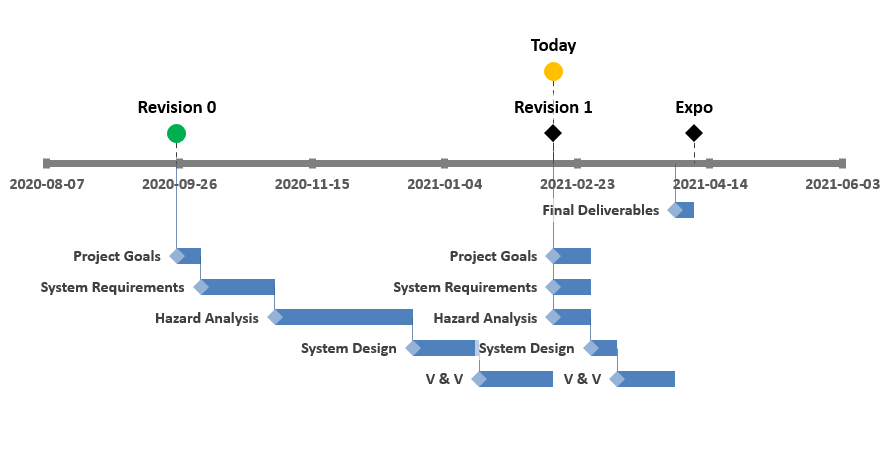
\includegraphics[width=\linewidth]{V_V/Roadmap.PNG}
  \caption{Project Road-map}
\end{figure}


\section{Components to be Tested}

\subsection{GUI}
    The GUI will be tested as follows: all reusable components will be assigned test cases to ensure their base functionality is validated. Then test cases for where these modules are used will also be included. Also, if not covered in the previously defined testing scenario, each `View' will also be assigned test cases to ensure all interactions provide the proper functionality to the user.
     \begin{itemize}
        \item Views
        \begin{itemize}
            \item ReadyView
            \begin{itemize}
                \item Will display current time, next dispense time, interactions to view current dispense times and request a manual dispensing of medication.
                \item Note: At this time, a successful manual dispense call will be simulated with a signal to the onboard LED. In the next revision, this button will be hidden behind a menu screen for saftey precautions. 
            \end{itemize}
            \item SetRTCView
            \begin{itemize}
                \item Consists of SetTimeModule for setting RTC time. Test included included in SetTime module test cases.
            \end{itemize}
            \item SetDispenseTimeView
            \begin{itemize}
                \item Consists of SetTimeModule for setting specified dispense time. Test included included in SetTime module test cases.
            \end{itemize}
            \item CurrentDispenseTimesView
            \begin{itemize}
                \item Consists of several DispenseTimeWidgets. Test included included in DispenseTimeWidgets module test cases.
            \end{itemize}
        \end{itemize}
        \item Reusable Modules
        \begin{itemize}
            \item  SetTime module
            \begin{itemize}
                \item  The SetTime Module is a reusable UI module that allows the users to create TimeStamps. The module consists of increase and decrease buttons for hour and minute, respectively. The component also allows the user to toggle A.M./P.M. This functionality will be the basis of correctness. On confirmation, the module creates a TimeStamp consisting of the hour, minute and am/pm value set by the user and passes it along to a custom callback defined elsewhere. This module is currently used in the SetRTCView and SetDispsenseSceen. Tests for the required functionality of these Views can be found in the last rows of the SetTime Module test case.

            \end{itemize}
            
            \item DispenseTimeWidget
            \begin{itemize}
                \item The DispenseTimeWidget is a reusable component specifically used in the ViewDispenseTimesView. It consists of a label describing the time period, a clock showing the set dispense time, and an `Edit' button that will allow the user to transition to the SetDispenseView for that period. 
            \end{itemize}
        \end{itemize}
        \end{itemize}
        
\subsection{Backend}
The backend system consists of call board interactions given changes in the monitored variables. This system will be tested by varying all values of the monitored variables and ensuring the proper functionality is conducted based off these changes.

\subsection{Mechanical}
The mechanical system will consist of motors, optical sensors, and a cutting device attached to a ball-screw. This system will be tested by sending signals from the backend to the mechanical system and ensuring that the correct psychical actions are taken and the correct output from the optical sensors are received on the backend.

\pagebreak
\section{Test Cases}

\subsection{GUI}

\subsubsection{Ready View}
\begin{tabularx}{\textwidth}{|X|X|X|p{0.22\textwidth}|p{0.22\textwidth}|X|}
        \hline
        \centering{\textbf{Test #}} \#     & \centering{\textbf{Desc}}     & \centering{\textbf{Inputs}}      & \centering{\textbf{Expected Outputs}}  & \centering{\textbf{Actual Outputs}}    & \centering{\textbf{Results}}   \\
        % View LOAD %
        \hline

        R01 & Test View creation & Ready View Object & 
        \begin{itemize}[leftmargin=*,topsep=0ex,parsep=0pt]
            \item Ready View displayed on device
            \item Digital Clock ticking from RTC.
            \item If available, next dispense time
        \end{itemize} & 
        \begin{itemize}[leftmargin=*,topsep=0ex,parsep=0pt]
            \item Ready View displayed on device
            \item Digital Clock ticking from RTC.
            \item If available, next dispense time displayed
        \end{itemize} & Pass
        
        \hline
        
        % View Dispense Times Button %
        \hline

        R02 & Test View Dispense Times Button & View Dispense Times Button press & Transition to ViewDispenseTimesView & Transition to ViewDispenseTimesView & Pass
        
        \hline
        
        % Request Manual Dispense Button %
        \hline

        R03 & Test Manual Dispense Button & Manual Dispense Button press & 
        \begin{itemize}[leftmargin=*,topsep=0ex,parsep=0pt]
            \item Dispensing Notification displayed
            \item Onboard LED lit.
        \end{itemize} & 
        Onboard LED lit. & Fail
        
        \hline
    \caption{Ready View Test Cases} %Caption here
    \end{tabularx}

\subsubsection{SetTime Module}

\begin{tabularx}{\textwidth}{|X|p{0.1\textwidth}|p{0.17\textwidth}|p{0.2\textwidth}|p{0.2\textwidth}|p{0.09\textwidth}|}
        \hline
        \centering{\textbf{Test #}} \#     & \centering{\textbf{Desc}}     & \centering{\textbf{Inputs}}      & \centering{\textbf{Expected Outputs}}  & \centering{\textbf{Actual Outputs}}    & \centering{\textbf{Results}}   \\
        
        %HOUR TESTS%
        \hline
        S01  & Testing increase hour button & Increase hour button press & 01 -$>$ 02 & 01 -$>$ 02 & Pass \\
        
        \hline
        S02  &  Testing decrease hour button & Decrease hour button press & 02 -$>$ 01 & 02 -$>$ 01 & Pass \\
        
        \hline
        S03  &  Testing increase hour button rollover &
       \begin{itemize}[leftmargin=*,topsep=0ex,parsep=0pt]
            \item Increase hour button press
            \item current hour = 12
        \end{itemize}

          & 12 -$>$ 01 & 12 -$>$ 01 & Pass \\
        
       \hline
        S04  &  Testing decrease hour button rollover & 
       \begin{itemize}[leftmargin=*,topsep=0ex,parsep=0pt]
            \item Decrease hour button press 
            \item current hour = 01
        \end{itemize}
        & 01 -$>$ 12 & 01 -$>$ 12 & Pass \\
        
        %MINUTE TESTS%
        \hline
        S05  &  Testing increase minute button & Increase minute button press & 00 -$>$ 01 & 00 -$>$ 01 & Pass \\
        
        \hline
        S06  &  Testing decrease minute button & Decrease minute button press & 01 -$>$ 00 &02 -$>$ 01 & Pass \\
        
        \hline
        S07  &  Testing increase minute button rollover & 
        \begin{itemize}[leftmargin=*,topsep=0ex,parsep=0pt]
            \item Increase minute button press 
            \item current minute = 59
        \end{itemize}
        & 59 -$>$ 00 & 59 -$>$ 00 & Pass \\
        
       \hline
        S08  &  Testing decrease minute button rollover & 
        \begin{itemize}[leftmargin=*,topsep=0ex,parsep=0pt]
            \item Decrease minute button press
            \item current minute = 00
        \end{itemize}
        & 00 -$>$ 59 & 00 -$>$ 59 & Pass \\
        
        %TOGGLE AM/PM TEST%
        \hline
        S09  &  Testing toggling of AM/PM & 
        \begin{itemize}[leftmargin=*,topsep=0ex,parsep=0pt]
            \item Toggle AM/PM button press
            \item  current state = AM
        \end{itemize}
        & AM -$>$ PM & AM -$>$ PM & Pass \\
        
        \hline
        S10  &  Testing toggling of AM/PM &
        \begin{itemize}[leftmargin=*,topsep=0ex,parsep=0pt]
            \item Toggle AM/PM button press
            \item   current state = PM
        \end{itemize}
        & PM -$>$ AM & PM -$>$ AM & Pass \\
        
        % RTC SET TEST%
        \hline
        S11  &  Testing confirm button for RTC Set & 
        \begin{itemize}[leftmargin=*,topsep=0ex,parsep=0pt]
            \item Confirm button press
            \item Current View is SetRTCView
            \item Time to set is 12:00:00 P.M
        \end{itemize} &
        \begin{itemize}[leftmargin=*,topsep=0ex,parsep=0pt]
            \item RTC = 12:00:00 P.M.
            \item View Transition -$>$ ReadyView
            \item ReadyView shown with RTC time
        \end{itemize} & 
        \begin{itemize}[leftmargin=*,topsep=0ex,parsep=0pt]
            \item RTC = 12:00:00 P.M.
            \item View Transition -$>$ ReadyView
            \item ReadyView shown with RTC time
        \end{itemize} &Pass \\
        \hline
        
        
        % Set Dispense TEST%
        \hline
        S12  &  Testing confirm button for Dispense Time & 
        \begin{itemize}[leftmargin=*,topsep=0ex,parsep=0pt]
            \item Confirm button press
            \item Current View is SetDispenseView
            \item Time to set is 12:00:00 P.M
        \end{itemize} &
        \begin{itemize}[leftmargin=*,topsep=0ex,parsep=0pt]
            \item Dispense time written to EEPROM.
            \item View Transition -$>$ ReadyView
            \item ReadyView shown with next dispense time
        \end{itemize} & 
        \begin{itemize}[leftmargin=*,topsep=0ex,parsep=0pt]
            \item Dispense time written to EEPROM.
            \item View Transition -$>$ ReadyView
            \item ReadyView shown with next dispense time
        \end{itemize} &Pass \\
        \hline
    \caption{SetTime Module Tests} %Caption here
    \end{tabularx}
    
    
\subsubsection{DispenseTimeWidget}

\begin{tabularx}{\textwidth}{|X|X|X|X|X|X|}
        \hline
        \centering{\textbf{Test #}} \#     & \centering{\textbf{Desc}}     & \centering{\textbf{Inputs}}      & \centering{\textbf{Expected Outputs}}  & \centering{\textbf{Actual Outputs}}    & \centering{\textbf{Results}}   \\
        \hline
         D01     & Testing Set Label     & Dispense period (Morning)     & Label shows ``Morning''   & Label shows ``Morning''     & Pass   \\
        \hline
         D02     & Testing Get Dispense Time for period (e.g. Morning)    &   12:00:00 P.M.     & Morning: 12:00:00 P.M.   & Morning: 12:00:00 P.M.    & Pass   \\
        \hline
         D03    & Testing Edit Button    &   Edit button press   & Transition to SetDispenseView with period information   & Transition to SetDispenseView with period information     & Pass   \\
        \hline
    \caption{DispenseTimeWidget} %Caption here
\end{tabularx}


\subsection{Backend}
\subsubsection{Ready State Test Cases}
\begin{tabularx}{\textwidth}{|X|X|X|X|X|X|}
        \hline
        Test \#     & Description     & Inputs      & Expected Outputs  & Actual Outputs    & Results   \\
        \hline
         RS01     & Testing when RTC reaches next Dispense Time     & RTC, Dispensing schedule     & Transition to Alarm State   & Transition to Alarm State     & Pass   \\
        \hline
         RS02     & Testing Manual Dispense Button     & Manual Dispense Button press     & Transition to Dispense State   & Transition to Dispense State     & Pass   \\
        \hline
    \caption{Ready State} %Caption here
\end{tabularx}

\subsubsection{Alarm State Test Cases}
\begin{tabularx}{\textwidth}{|X|X|X|X|X|X|}
        \hline
        Test \#     & Description     & Inputs      & Expected Outputs  & Actual Outputs    & Results   \\
        \hline
         A01     & Testing Notification System     & Ready to Alarm transition argument received     & Alarm to sound. Dispense button to appear.   & Alarm to sound. Dispense button to appear.     & Pass   \\
        \hline
         A02     & Testing Dispense Button Press     & Dispense Button press     & Transition to Dispense State   & Transition to Dispense State     & Pass   \\
        \hline
         A03     & Testing Timeout     & Alarm untouched for 5 minutes     & Transition to Timeout State   & Transition to Timeout State     & Pass   \\
        \hline
    \caption{Alarm State} %Caption here
\end{tabularx}

\subsubsection{Alarm Timeout State Test Cases}
\begin{tabularx}{\textwidth}{|X|X|X|X|X|X|}
        \hline
        Test \#     & Description     & Inputs      & Expected Outputs  & Actual Outputs    & Results   \\
        \hline
         AT01     & Testing Dispense Button    & Dispense Button press     & Transition to Dispense State   & Transition to Dispense State     & Pass   \\
        \hline
    \caption{Alarm Timeout State} %Caption here
\end{tabularx}

\subsubsection{Dispense State Test Cases}
\begin{tabularx}{\textwidth}{|X|X|X|X|X|X|}
        \hline
        Test \#     & Description     & Inputs      & Expected Outputs  & Actual Outputs    & Results   \\
        \hline
         DS01     & Registering a Dispense    & Dispensing mechanism, sensors, dispense button press     & Pill sachet dispenses. Transition to Wait for Collection State.   & Pill sachet dispenses. Transition to Wait for Collection State.     & Pass   \\
        \hline
         DS02     & Testing Dispensing Time   &  Dispense Button press     & Sachet dispensed in under 15 seconds   & Sachet dispensed in under 15 seconds & Pass   \\
        \hline
         DS03     & Testing Dispensing Accuracy     & Dispense Button press     & Correct number of sachets dispensed   & Correct number of sachets dispensed     & Pass   \\
        \hline
    \caption{Dispense State} %Caption here
\end{tabularx}

\subsubsection{Wait for Collection State Test Cases}
\begin{tabularx}{\textwidth}{|X|X|X|X|X|X|}
        \hline
        Test \#     & Description     & Inputs      & Expected Outputs  & Actual Outputs    & Results   \\
        \hline
         W01     & Testing if Pills have been Removed    & Sensor in pill collection area     & Transition to Adherence Update State   & Transition to Adherence Update State     & Pass   \\
        \hline
    \caption{Wait for Collection State} %Caption here
\end{tabularx}

\subsubsection{Adherence Update State Test Cases}
\begin{tabularx}{\textwidth}{|X|X|X|X|X|X|}
        \hline
        Test \#     & Description     & Inputs      & Expected Outputs  & Actual Outputs    & Results   \\
        \hline
         AU01     & Testing to determine if Adherence Data has been written to Non-Volatile Memory    & N/A     & N/A   & N/A     & N/A   \\
        \hline
    \caption{Adherence Update State} %Caption here
\end{tabularx}

\subsection{Hardware Test Cases}
\begin{tabularx}{\textwidth}{|X|X|X|X|X|X|}
        \hline
        Test \#     & Description     & Inputs      & Expected Outputs  & Actual Outputs    & Results   \\
        \hline
         H01     & Testing Machine Loading  & Pill strip loaded into machine, load new pill strip button press    & Internal sensor send a 1 in under 15 seconds saying sachet is loaded  & N/A & N/A   \\
        \hline
         H02     & Manual Pill Dispense   & Manual dispense button pressed  &  Opened pill sachet is dispensed and dispensing area sensor triggered in under 15 seconds  & N/A & N/A  \\
        \hline
         H03     & Scheduled Pill Dispense   & Scheduled time passes and Dispense button pressed  &  Opened pill sachet is dispensed and dispensing area sensor triggered in under 15 seconds  & N/A & N/A  \\
        \hline
         H04     & Sachet Removed from Dispensing Area   & User removing pill sachet from dispensing area  & Dispensing area sensor sends a 0  & N/A & N/A  \\
        \hline
%         05     &  Unexpected Object in Dispensing Area  &   &    & N/A & N/A  \\
%        \hline
    \caption{Hardware Testing} %Caption here
\end{tabularx}


\section{Beyond Testing}

\subsection{Code Walk-through and Code Reviews}
After a feature was considered complete and ready to review, a merge request was made through GitLab, and 2 reviewers who had not worked on the feature are assigned to the request. All three members would then engage in a code review where the author would explain functionality and the implementation at hand. The reviewers would then ask questions to challenge the authors implementation. Once all commits are agreed upon, the request would be merged into the main branch.

\subsection{Results of Peer Reviews}

The previously mentioned code review process has also been used for much of the development of the rest of the project. This style of review has allowed for further brainstorming of solutions and has allowed for different solutions to be viewed from different perspectives.


\pagebreak
\section{Traceability Matrix}
The following traceability matrix may be used to map the above test cases to the corresponding requirements they cover. For the purposes of readability the abbreviations FR and NFR have been used for Functional and Non-functional requirements (ex. FR1 corresponds to function requirement 1, and NFR3 to non-functional requirement 3). 

\begin{longtable}{|p{0.08\textwidth}|p{0.6\textwidth}|p{0.08\textwidth}|p{0.12\textwidth}|}
        \hline
        Req \# & Description & Test \# & Status \\ \hline
%-----------------------
FR1 & The dispenser will dispense sachet(s) with 99.9\% effectiveness. 
& N/A & Incomplete       \\ \hline
%-----------------------
FR2    & The dispenser must dispense the correct sachet(s) at the correct time in accordance with a set schedule. 
& RS01 \newline 
A02 \newline
AT01 \newline
DS03 \newline
H03
& Pass \newline
Pass \newline
Pass \newline
Pass \newline
DNC
\\ \hline
%-----------------------
FR3    & The dispenser will keep track of how many sachets are yet to be dispensed and will tell the user when it is nearly or entirely empty.
& N/A  & Incomplete    \\ \hline

FR4    & The dispenser will only allow the user to retrieve the medication when it is safe to do so. 
&  H04  &  DNC \\ \hline
%-----------------------
FR5 & The dispenser must verify that the medication was successfully dispensed. 
& DS01 & Pass    \\ \hline
%-----------------------
FR6    & The dispenser must know if and when a dispensed sachet is collected/retrieved by the user and records the event. 
& W01 \newline 
AU01 \newline
H04
& Pass \newline
DNC\newline
DNC \\ \hline
%-----------------------
FR7    & The dispenser must keep an accurate real-time clock. 
& R01 & Pass      \\ \hline
%-----------------------
FR8    & The dispenser must be able to hold and dispense McKesson PACMED pill sachets. 
& H01 & DNC \\ \hline
%-----------------------
FR9    & The dispenser must notify the user when it is time to take a scheduled medication. 
& A01 & Pass \\ \hline
%-----------------------
FR10   & The dispenser must allow the user to manually dispense sachets as necessary. 
& R03 \newline
RS02
H02
& Fail \newline
Pass \newline
DNC \\ \hline
%-----------------------
FR11   & The dispenser must allow the user to update the real-time clock as necessary. 
& S01 \newline 
S02 \newline
S03 \newline
S04 \newline
S05 \newline
S06 \newline
S07 \newline
S08 \newline
S09 \newline
S10 \newline
S11 \newline
& Pass \newline
Pass \newline
Pass \newline 
Pass \newline 
Pass \newline 
Pass \newline 
Pass \newline 
Pass \newline 
Pass \newline 
Pass \newline 
Pass \newline 
\\ \hline
%-----------------------
FR12   & The dispenser must allow the user to update the current dispensing schedule as necessary.
& R02 \newline 
S01 \newline 
S02 \newline
S03 \newline
S04 \newline
S05 \newline
S06 \newline
S07 \newline
S08 \newline
S09 \newline
S10 \newline
S12 \newline
D01 \newline
D02 \newline
D03 \newline
& Pass \newline
Pass \newline
Pass \newline
Pass \newline 
Pass \newline 
Pass \newline 
Pass \newline 
Pass \newline 
Pass \newline 
Pass \newline 
Pass \newline 
Pass \newline 
Pass \newline 
Pass \newline 
Pass \newline 
 \hline
%-----------------------
FR13   & The dispenser must store adherence data on local non-volatile memory. 
&  N/A & Incomplete         \\ \hline
%-----------------------
FR14   & The user must be able to see adherence data via the user interface or through a direct connection to the device (ex. USB). 
&  N/A & Incomplete         \\ \hline
%-----------------------
FR15   & The dispenser must not damage any pills during the dispensing process. 
&  N/A & Incomplete         \\ \hline
%-----------------------
FR16   & All moving parts/hazards within the device must be safely concealed to prevent user injury. 
&  N/A & Incomplete         \\ \hline
%-----------------------
FR17   & The system must be able to identify when a jam occurs and provide instruction to the user. 
&  N/A & Incomplete         \\ \hline
%-----------------------
NFR1   & The dispenser shall dispense a sachet within a reasonable time period ($<$ 15s). 
& DS02 & Pass \\ \hline
%-----------------------
NFR2   & The dispenser shall be easy to set-up with intuitive instructions. 
&  N/A & Incomplete         \\ \hline
%-----------------------
NFR3   & The dispenser shall appear aesthetically pleasing. 
&  N/A & Incomplete         \\ \hline
%-----------------------
NFR4   & The dispenser shall consume minimal power. 
&  N/A & Incomplete         \\ \hline
%-----------------------
NFR5   & The dispenser be small enough to fit on a counter-top. 
&  N/A & Incomplete         \\ \hline
%-----------------------
NFR6   & The dispenser must enter a sleep state if it has had no user interaction for longer than 2 minutes. 
&   N/A & Incomplete         \\ \hline
%-----------------------
\caption{Requirement Traceability Matrix} %Caption here
\end{longtable}

\end{document}

